\chapter{Topological Data Analysis}

This chapter documents our topological data analysis of the two point clouds. Our main tool is the GUDHI library in Python. \cite{gudhi:manual} Each section is dedicated to a step of the analysis. Within each section, we
\begin{itemize}
    \item Describe the computational steps employed by GUDHI,
    \item Explain the choice of any tuning parameters,
    \item Present results of the analytic step for our dataset.
\end{itemize}

\section{Filtrations}
The atoms of algebraic topology are chain complexes (\cref{chaincomplex}), essentially sequences of algebraic information. In our analysis, we use the Vietoris-Rips complex (\cref{vrcomplex}). The Vietoris-Rips complex packages the information from a point cloud in a format that is computable.
\\\\
A filtration (\cref{filtration}) is a nested collection of algebraic objects, in our case Vietoris-Rips complexes. Thus, the goal of this step is to compute the Vietoris-Rips filtration (\cref{vrfiltration}) following the GUDHI Tutorial: \cite{gudhi_tutorial_complexes}.
\\\\
There are two tuning parameters in this process: \textit{maximum edge length} and \textit{maximum dimension}. 
\\\\
The maximum edge length, measured as a percentage of the diameter of the point cloud, represents the largest Vietoris-Rips complex included in the filtration. We selected the largest maximum edge length that did not crash the program, which was 15\%.
\\\\
The maximum dimension is the dimension of Vietoris-Rips complexes included in the filtration. We set a maximum dimension of 3, as dimension 0, 1, and 2 features are usually the only ones that are human-interpretable.
\\\\
The filtration for both the control and CTE images use all 1000 points from the point cloud. The control filtration contained 24 million simplices and the CTE filtration contained 33 million simplices.

\section{Barcodes and Diagrams}
Persistence modules (\cref{persistencemodule}) convert the information of filtrations to a format compatible with the tools of linear algebra. This has two significant consequences:
\begin{itemize}
    \item The information stored in a filtration can be computed efficiently.
    \item That information can be decomposed as a sum of its parts via the structure theorem.
\end{itemize}
The decomposition of a persistence module is represented by persistence barcodes and diagrams. The two are different visualisations of the same information, and we followed the GUDHI Tutorial: \cite{gudhi_tutorial_persistence}.
\\\\
Computing the persistence module is the most expensive step of TDA. Prior decisions (for instance, how many points of a point cloud to subsample) were made with the persistence modules in mind.
\\\\
The output of a persistence module computation is a list of features with the following information: birth time, death time, and dimension. The birth time is the step at which that feature first appeared. The death time is the step at which that feature was filled in by a higher-dimensional feature. Features that do not die are assigned a death time of $+\infty$. 
\\\\
Persistence barcodes are a histogram of every feature along the vertical axis. The horizontal axis colours the feature from its birth time to its death time. Persistence diagrams plot the birth time of each feature along the $x$ axis and the death time of each feature along the $y$ axis. In both, the dimension of the feature is colour-coded.
\\\\
The persistence barcodes and diagrams of both the control and CTE brains are presented in \cref{fig:persistence}.

\begin{figure}[htbp]
  \centering
  % Row 1
  \begin{subfigure}[b]{0.48\textwidth}
    \centering
    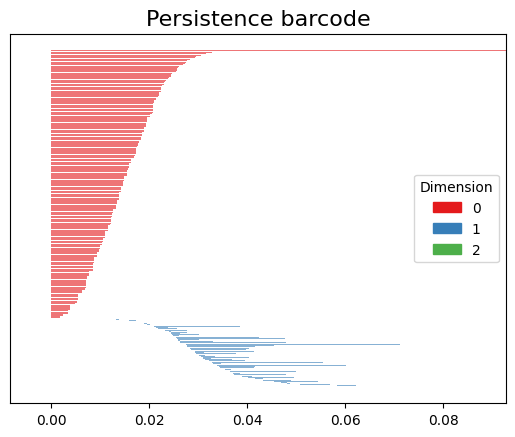
\includegraphics[width=\linewidth]{control_barcode.png}
    \caption{Persistence barcode of the control brain.}
    \label{fig:first}
  \end{subfigure}
  \hfill
  \begin{subfigure}[b]{0.48\textwidth}
    \centering
    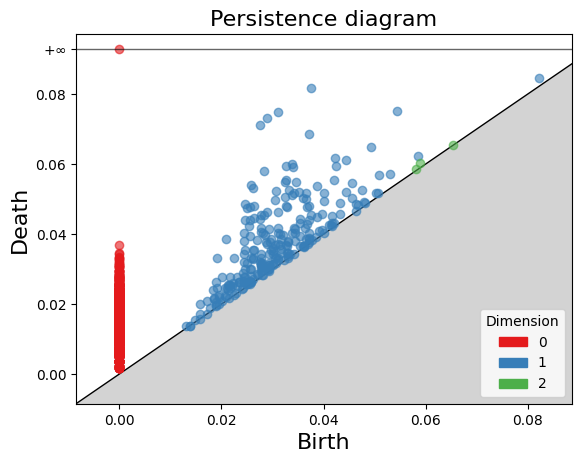
\includegraphics[width=\linewidth]{control_diagram.png}
    \caption{Persistence diagram of the control brain.}
    \label{fig:second}
  \end{subfigure}

  \vspace{1em}

  % Row 2
  \begin{subfigure}[b]{0.48\textwidth}
    \centering
    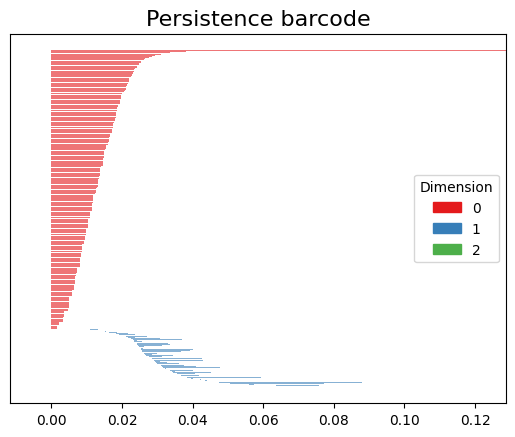
\includegraphics[width=\linewidth]{cte_barcode.png}
    \caption{Persistence barcode of the CTE brain.}
    \label{fig:third}
  \end{subfigure}
  \hfill
  \begin{subfigure}[b]{0.48\textwidth}
    \centering
    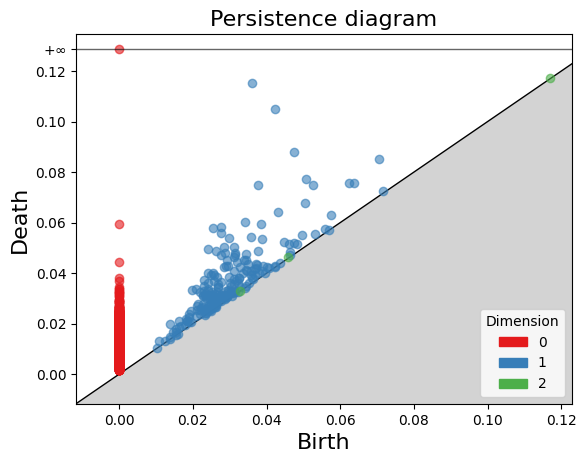
\includegraphics[width=\linewidth]{cte_diagram.png}
    \caption{Persistence diagram of the CTE brain.}
    \label{fig:fourth}
  \end{subfigure}

  \caption{Persistence barcodes and diagrams of our data.}
  \label{fig:persistence}
\end{figure}

\section{Comparison}\label{comparison}
Our comparison of persistence modules involves two questions: (i) are there any differences between the two brains? and (ii) can we locate and visualise those differences?
\subsection{Are there any differences?}
We need to compare diagrams/barcodes, which are derived from the persistence modules. We select two metrics: the bottleneck distance (\cref{bottleneckdist}) and the Wasserstein distance (\cref{wassersteindist}). Both distances attempt to match elements of the barcodes/diagrams under comparison. In the bottleneck distance, only the single greatest mismatch is considered, whereas in the Wasserstein distance all mismatches are weighted and summed.
\\\\
Both distances are measured as a percentage of the point cloud diameter. Unlike familiar statistical tests, the $t$-test, $\chi^2$ test, etc, the bottleneck and Wasserstein distances do not have an analogous notion of hypothesis testing. Thus, to make comparisons, we construct \textit{resampled} versions of both the control and CTE point clouds by selecting a different subsample of point to the original. 
\\\\
Another nuance is that persistence modules contain multiple types of topological data, graded by dimension. Thus, comparisons must be made on a dimension-by-dimension basis.
\\\\
We present comparisons of the control vs CTE brain, and the control vs (control) resample and the CTE vs (CTE) resample, for each dimension, for both the bottleneck and Wasserstein distances, in \cref{tab:bottleneck} and \cref{tab:wasserstein}.
\begin{table}[h]
\centering
\begin{tabular}{|c|c|c|c|}
\hline
 & Control vs CTE & Control vs Resample & CTE vs Resample \\ \hline
Dimension 0 & 2.274 & 0.375 & 0.999 \\ \hline
Dimension 1 & 3.329 & 0.815 & 2.511 \\ \hline
Dimension 2 & 0.068 & 0.068 & 0.075 \\ \hline
\end{tabular}
\caption{Bottleneck Distance (\% of point cloud diameter)}
\label{tab:bottleneck}
\end{table}

\begin{table}[h]
\centering
\begin{tabular}{|c|c|c|c|}
\hline
 & Control vs CTE & Control vs Resample & CTE vs Resample \\ \hline
Dimension 0 & 0.142 & 0.040 & 0.034 \\ \hline
Dimension 1 & 0.200 & 0.114 & 0.168 \\ \hline
Dimension 2 & 0.052 & 0.034 & 0.057 \\ \hline
\end{tabular}
\caption{Wasserstein Distance (\% of point cloud diameter)}
\label{tab:wasserstein}
\end{table}
\noindent
We interpret the results of \cref{tab:bottleneck} and \cref{tab:wasserstein} dimension-by-dimension.
\\\\
Dimension $0$ features are born as individual points and die when they are connected with another point. In both \cref{tab:bottleneck} and \cref{tab:wasserstein} we see that the Control vs CTE distance is large relative to the resampled distances. Our interpretation of this is that many of the points in the CTE brain are isolated for `longer', so there are greater distances between them.
\\\\
Dimension $1$ features are born as lines and die when they are filled in as a triangle. In \cref{tab:bottleneck} we see that the Control vs CTE distance is large relative to the resampled distances, whereas the difference is more modest in \cref{tab:wasserstein}. This suggests that (relatively) few extreme features are driving the overall difference. These features are likely to represent the number and size of holes, as the triangles fill in the gaps created by the surrounding points.
\\\\
Dimension $2$ features are born as triangles and die when they are filled in as a tetrahedron. In both \cref{tab:bottleneck} and \cref{tab:wasserstein} we see that the Control vs CTE distance is similar to the resampled distances, so any observed dimension $2$ features are likely just noise. Intuitively, this makes sense as the images are \textit{flat} sections of a brain, which obscures any cavities.
\subsection{Where are the differences?}
Now our approach differs from many applications of TDA in the literature, where it is common to feed the features from TDA into a machine learning algorithm, for instance in \cite{qaiser2019fast}.
\\\\
We prefer to visualise the features of the point cloud that contribute most to the Wasserstein distance. We implement this procedure for the dimension 1 features, as they have the clearest interpretation.
\\\\
To do this, we rank all dimension 1 features in the CTE brain by their contribution to the Wasserstein distance, highlight the dimension 1 simplex (line) that births the feature, and shade in the dimension 2 simplex (triangle) that kills the feature.
\\\\
A histogram of the contributions to the Wasserstein distance of the dimension 1 features is plotted in \cref{fig:hist}.
\begin{figure}[H]
  \centering
  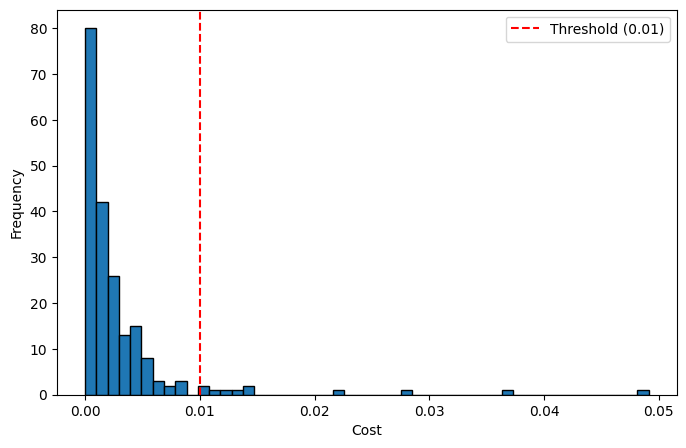
\includegraphics[width=0.6\textwidth]{his.png}
  \caption{Histogram of Dimension 1 Features.}
  \label{fig:hist}
\end{figure}
\noindent
On visual inspection, we choose a threshold at 0.01 to represent the \textit{greatest} contributors to the Wasserstein distance. This decision was also made to keep the number of features relatively small (11, in this case).
\\\\
The birth dimension 1 simplex (line) and death dimension 2 simplex (triangle) corresponding to the 11 features above the threshold in \cref{fig:hist} are plotted in \cref{fig:features}.
\begin{figure}[H]
  \centering
  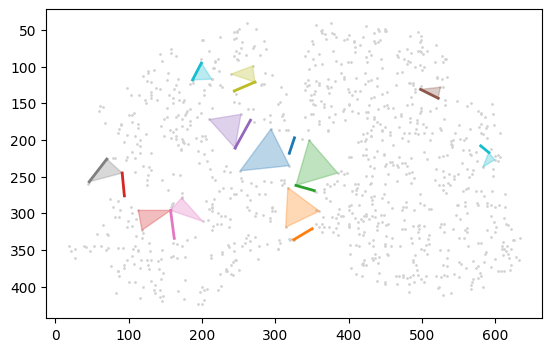
\includegraphics[width=0.75\textwidth]{cte_features.png}
  \caption{CTE Point Cloud with Highlighted Features.}
  \label{fig:features}
\end{figure}
\noindent



